\documentclass[tikz,border=0pt,11pt]{standalone}
\usepackage[T1]{fontenc}
\usepackage[utf8]{inputenc}
\usepackage{lmodern,amsmath,amssymb}
\usepackage[swedish]{babel}
\usetikzlibrary{arrows.meta,calc,positioning,decorations.pathmorphing,decorations.pathreplacing,patterns,shadings}
\definecolor{navy}{HTML}{102F40}
\definecolor{teal}{HTML}{147D78}
\definecolor{lightteal}{HTML}{E6F1ED}
\definecolor{gold}{HTML}{B88B3B}
\definecolor{palegold}{HTML}{F7EEDB}
\definecolor{rust}{HTML}{B6533B}
\definecolor{palerust}{HTML}{FAEAE4}
\definecolor{paper}{HTML}{F7F5EE}
\definecolor{muted}{HTML}{5B6D72}
\definecolor{line}{HTML}{D6DED8}
\renewcommand{\familydefault}{\sfdefault}
\newcommand{\atom}[5]{\shade[ball color=#3!70] (#1,#2) circle (#5);\node[text=white,font=\bfseries\small] at (#1,#2){#4};}
\newcommand{\water}[3]{\begin{scope}[shift={(#1,#2)},scale=#3]\draw[navy!45,line width=2pt] (-.3,.22)--(0,0)--(.3,.22);\atom{0}{0}{rust}{O}{.22}\atom{-.3}{.22}{teal}{H}{.15}\atom{.3}{.22}{teal}{H}{.15}\end{scope}}
\newcommand{\panel}[4]{\filldraw[fill=white,draw=line,rounded corners=5pt] (#1,#2) rectangle ++(#3,#4);}
\newcommand{\note}[4]{\node[txt,text width=#3cm] at (#1,#2){#4};}
\tikzset{txt/.style={anchor=north west,align=left,text=navy,font=\small},
 head/.style={anchor=west,text=navy,font=\bfseries\large},
 label/.style={align=center,text=navy,font=\small},
 smalllabel/.style={align=center,text=muted,font=\footnotesize},
 arrow/.style={-{Latex[length=2.5mm,width=1.8mm]},line width=1.2pt,draw=teal},
 goldarrow/.style={-{Latex[length=2.5mm]},line width=1.2pt,draw=gold},
 rustarrow/.style={-{Latex[length=2.5mm]},line width=1.2pt,draw=rust},
 dashedarrow/.style={arrow,dashed},
 badge/.style={fill=lightteal,rounded corners=3pt,text=teal,font=\bfseries\small,inner sep=5pt}}
\begin{document}
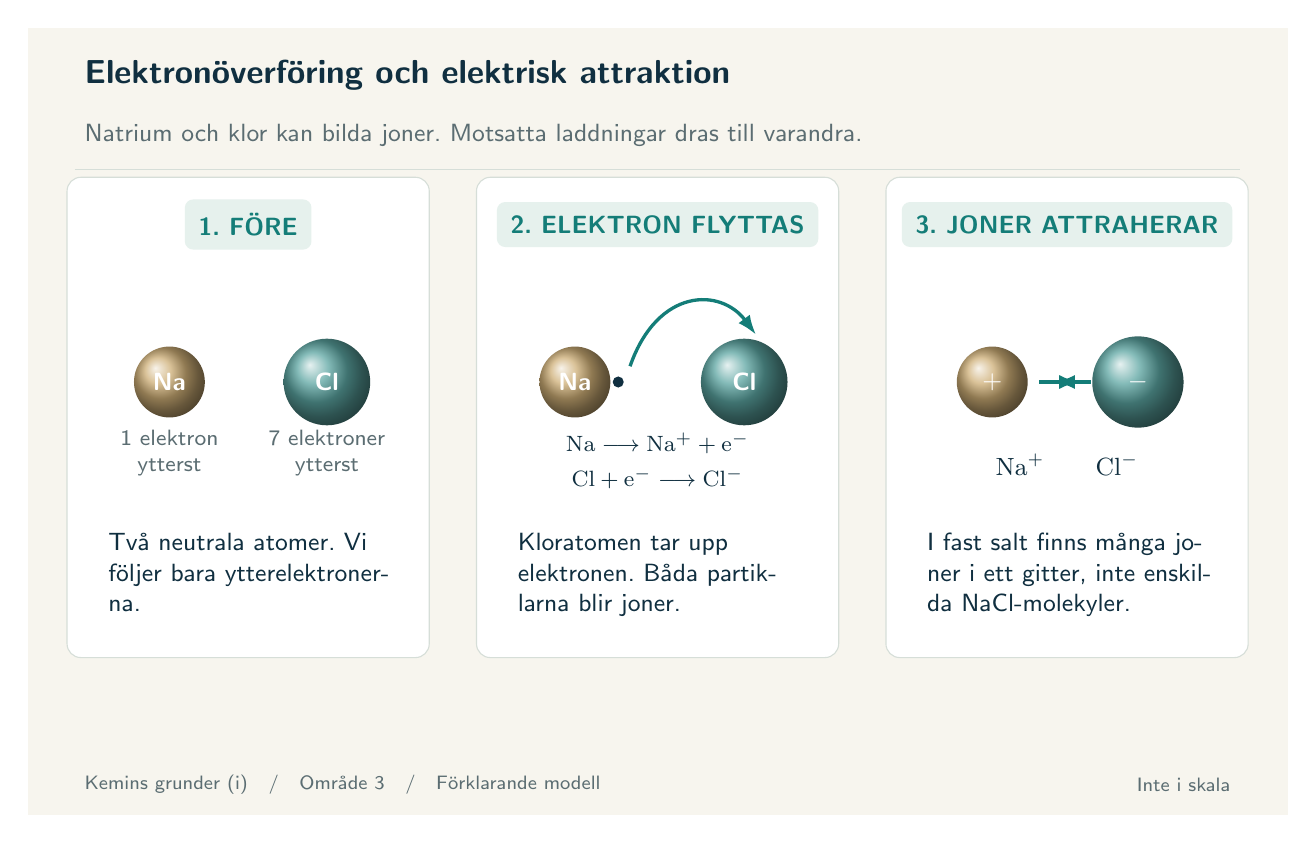
\begin{tikzpicture}[x=1cm,y=1cm]
\path[use as bounding box] (0,0) rectangle (16,10);
\fill[paper] (0,0) rectangle (16,10);
\node[head] at (.6,9.4){Elektronöverföring och elektrisk attraktion};
\note{.6}{8.9}{14.8}{\textcolor{muted}{Natrium och klor kan bilda joner. Motsatta laddningar dras till varandra.}}
\draw[line] (.6,8.2)--(15.4,8.2);

\panel{.5}{2}{4.6}{6.1}\panel{5.7}{2}{4.6}{6.1}\panel{10.9}{2}{4.6}{6.1}
\node[badge] at (2.8,7.5){1. FÖRE};\node[badge] at (8,7.5){2. ELEKTRON FLYTTAS};\node[badge] at (13.2,7.5){3. JONER ATTRAHERAR};
\atom{1.8}{5.5}{gold}{Na}{.45}\atom{3.8}{5.5}{teal}{Cl}{.55}
\node[smalllabel,text width=1.8cm] at (1.8,4.6){1 elektron\\ytterst};\node[smalllabel,text width=1.8cm] at (3.8,4.6){7 elektroner\\ytterst};
\atom{6.95}{5.5}{gold}{Na}{.45}\atom{9.1}{5.5}{teal}{Cl}{.55}
\fill[navy] (7.5,5.5) circle(.07);\draw[arrow] (7.65,5.7).. controls(8,6.7) and (8.8,6.7)..(9.25,6.1);
\node[label,font=\footnotesize] at (8,4.5){$\mathrm{Na\longrightarrow Na^++e^-}$\\[3pt] $\mathrm{Cl+e^-\longrightarrow Cl^-}$};
\atom{12.25}{5.5}{gold}{$+$}{.45}\atom{14.1}{5.5}{teal}{$-$}{.58}
\draw[arrow] (12.85,5.5)--(13.35,5.5);\draw[arrow] (13.5,5.5)--(13.05,5.5);
\node[label] at (13.2,4.45){$\mathrm{Na^+\qquad Cl^-}$};
\note{.9}{3.7}{3.8}{Två neutrala atomer. Vi följer bara ytterelektronerna.}
\note{6.1}{3.7}{3.8}{Kloratomen tar upp elektronen. Båda partiklarna blir joner.}
\note{11.3}{3.7}{3.8}{I fast salt finns många joner i ett gitter, inte enskilda NaCl-molekyler.}\node[anchor=west,text=muted,font=\scriptsize] at (.6,.38){Kemins grunder (i)\quad /\quad Område 3\quad /\quad Förklarande modell};
\node[anchor=east,text=muted,font=\scriptsize] at (15.4,.38){Inte i skala};
\end{tikzpicture}\end{document}
